%Note di Ingegneria del Software
%Sommario: SOLID

\cornell{SOLID}{Robert Martin (Il prof. Cardin consiglia il libro "Clean Code")\\
Dà dei dettami per avere un codice pulito, comprensibile e più possibile manutenibile.\\
Ovvero offre delle best practice per avere codice flessibile, robusto e riusabile.\\
\begin{description}
        \item[S]ingle Responsibility
        \item[O]pen/Closed Principle
        \item[L]iskov Substitution Principle
        \item[I]nterface Segregation
        \item[D]ependency Inversion
\end{description}\\
Solitamente i primi 3 sono considerati i più importanti}

\cornell{Single Responsibility}{Basato sul concetto di \textbf{Coesione}.\\
Tipi che insieme vanno a comporre una funzionalità (o che comunque sono usati insieme), dovrebbero evolvere/cambiare insieme.\\
Un modulo dovrebbe avere una sola ragione per cambiare.\\
Concetto antitetico: \textbf{Accoppiamento} (dove si ha che due o più classi devono cambiare anche se non sono usate assieme)\\
In caso di cambiamenti ad una classe, l'accoppiamento ci forzerebbe a cambiare alcune (o tutte) le classi collegate}

\cornell[Memo]{Dipendenze e Transitività}{Le dipendenze \textbf{non sono transitive}\\
$A \longrightarrow B \land B \longrightarrow C \notimplies A \longrightarrow C$}

\cornell{Esempio}{ 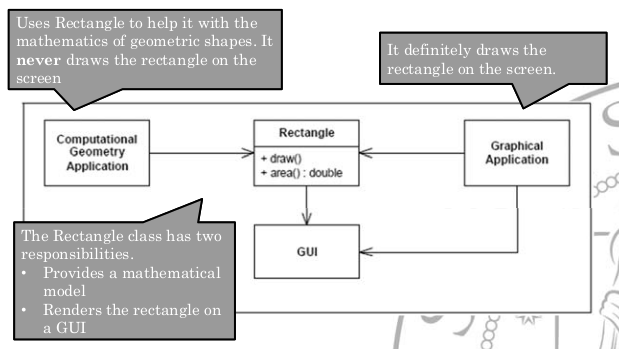
\includegraphics[scale=0.5]{images/76.png}\\
Alla "Computational Geometry Application" non dovrebbero interessare eventuali cambiamenti al metodo \texttt{draw()} di Rectangle, ma l'accoppiamento ci costringe ad effettuare comunque cambiamenti a "Computational Geometry Application" quando Rectangle viene aggiornato alla nuova versione.\\
La soluzione è dividere le responsabilità:\\
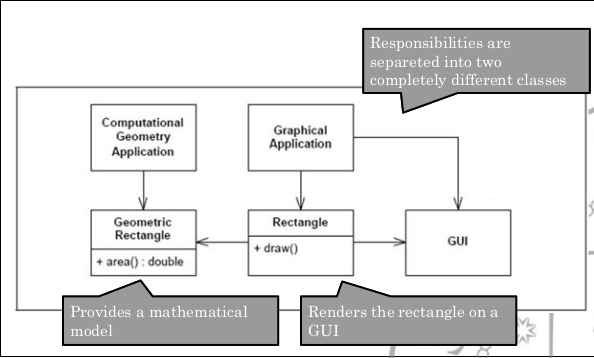
\includegraphics[scale=0.5]{images/77.png}}

\cornell{Cos'è una Responsibility}{È un "asse di cambiamento" che va interpretato a seconda del contesto.\\
Ad esempio:\\
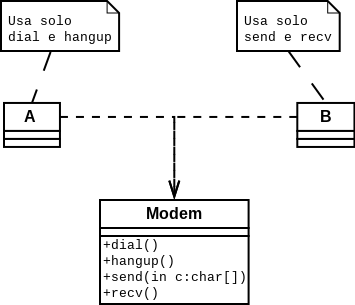
\includegraphics[scale=0.5]{images/78.png}}
\cornell{Tentativo}{Proviamo ad applicare lo stesso principio usato in rectangle e separiamo i 4 metodi in 4 classi diverse. Ci ritroviamo con una situazione del tipo:
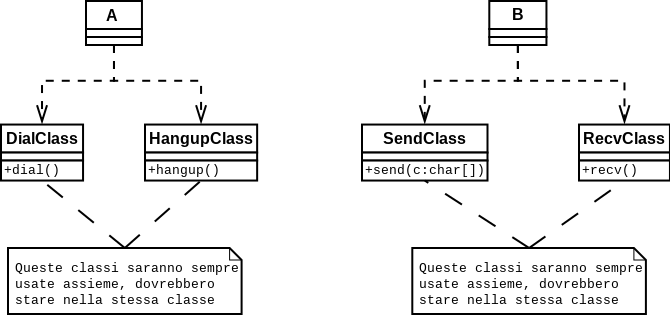
\includegraphics[scale=0.4]{images/79.png}\\
Ho perso coesione e mi ritrovo con degli accoppiamenti non previsti. In questo contesto la classe Modem aveva 2 assi di cambiamento (e non 4), cioè le funzione di "Gestione della connessione" (dial e hangup) e le funzioni di comunicazione (send e recv).}
\cornell{Assi di cambiamento}{Ovviamente tale classe non ha due assi di cambiamento in senso assoluto, in questa situazione ad esempio:\\
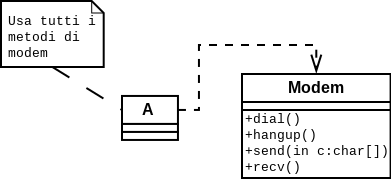
\includegraphics[scale=0.5]{images/80.png}\\
La classe Modem è coesa e non è necessaria separazione delle responsabilità.}

\cornell{La soluzione corretta}{Nel caso esaminato, in cui A usa le funzioni di gestione connessione e B quelle di comunicazione, la soluzione migliore è la seguente:\\
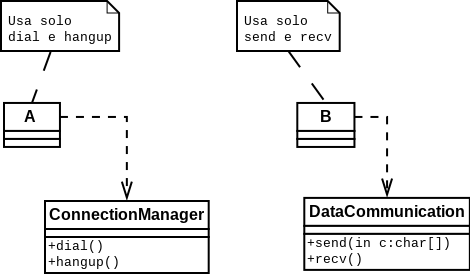
\includegraphics[scale=0.5]{images/81.png}}

\cornell{Domanda}{E se avessi una situazione del genere?\\
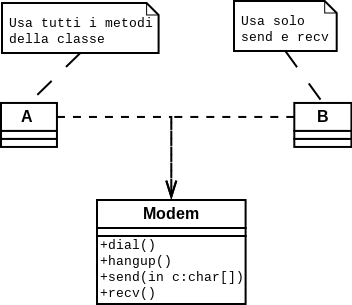
\includegraphics[scale=0.5]{images/82.png}\\
Dobbiamo ricordarci che il principio funziona in casi astratti, quindi possiamo fare uso delle interfacce per avere il risultato migliore:\\
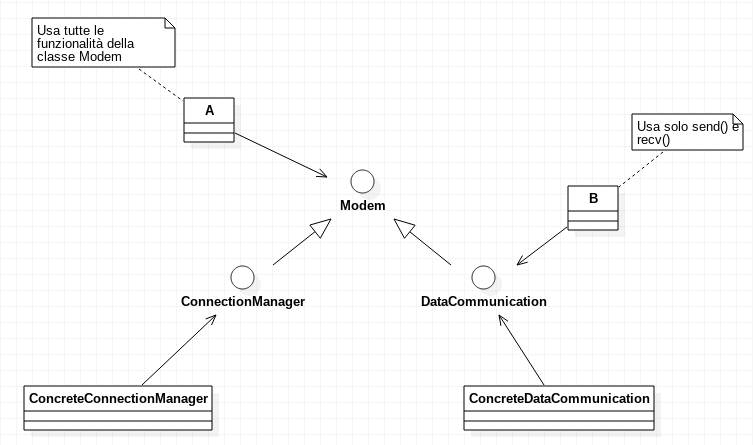
\includegraphics[scale=0.4]{images/83.png}}

\cornell{Open/Close Principle}{Le entità software dovrebbero essere \begin{itemize}
\item Aperte all'estensione
\item Chiuse alla modifica
\end{itemize}\\
I comportamenti di un software vengono quindi modificati \textbf{aggiungendo} codice e non modificando il codice esistente (a parte in caso di bug)\\
Questo principio può essere realizzato tramite \textbf{astrazione} (di tipo puro, cioè tramite interfacce).}
\cornell{Esempio}{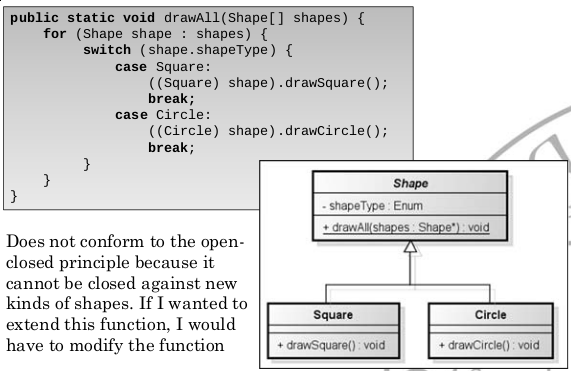
\includegraphics[scale=0.4]{images/84.png}\\
Se guardiamo il codice, DrawAll fa uso di cast, oltre alla presenza di un enum "shapeType" che limita l'estensibilità della gerarchia. Se voglio aggiungere una nuova forma, dovrò andare a modificare "Shape".}

\cornell{Riadattamento}{È possibile riadattare la gerarchia all'open-close principle creando un metodo \texttt{draw()} astratto che viene sovrascritto dalle varie forme.\\
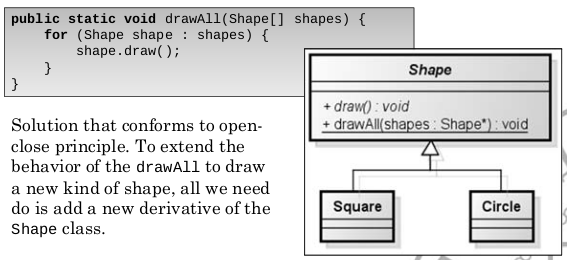
\includegraphics[scale=0.5]{images/85.png}\\
In questo modo evito le "cascate di cambiamenti"}

\cornell{Note sull'OCP}{\begin{itemize}
\item Non è un principio assoluto: è impossibile avere un programma 100\% chiuso, è necessario essere un po' strategici
\item La chiusura si può ottenere per astrazione: tramite ereditarietà e polimorfismo
\item La chiusura si può ottenere anche in modo "data-driven": usando strutture esterne.
\end{itemize}}

\cornell{Dettami di OCP}{Sono quelli standard della Programmazione OO:\begin{itemize}
\item Le variabili membro devono essere tutte private
\item Non si usano mai variabili globali
\item La RTTI è pericolosa
\end{itemize}}

\cornell{Liskov Substitution Principle}{Funzioni che usano puntatori o riferimenti a classi base, devono essere in grado di usare oggetti di classi derivate in modo trasparente.\\
Solitamente violare questo principio porta anche a violare l'Open/Close Principle.\\
Anche qui è necessario fare molta attenzione a come vengono usate le classi:\\
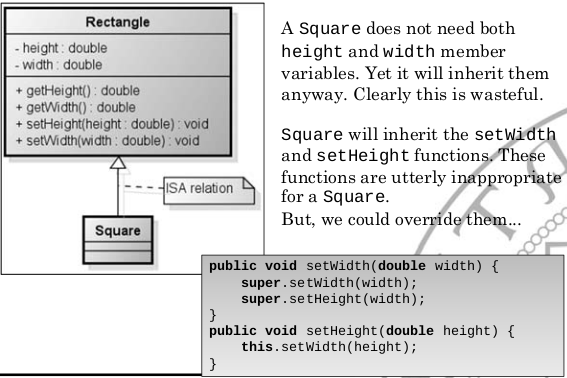
\includegraphics[scale=0.5]{images/86.png}}

\cornell{Qual'è il problema}{Dopo aver considerato questa gerarchia, vediamo il seguente test:\\
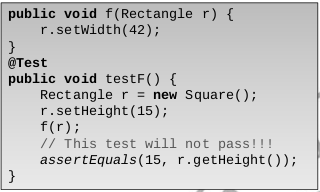
\includegraphics[scale=0.6]{images/87.png}\\
Il test non passa perchè nonostante Square sia un caso particolare di Rectangle, la precondizione di setWidth in square è più stringente di quella in Rectangle (infatti va ad effettuare anche un setHeight)\\
Se usate in questo modo, il codice del test richiede che Square e Rectangle siano due classi completamente separate.}

\cornell{Cosa se ne evince}{La validità di un modello può essere valutata solo in funzione del modo in cui tale modello è usato.\\
Un altro consiglio è quello di non usare ereditarietà allo scopo di condividere del codice: ciò che veramente contano sono le operazioni che possono essere usate dai client esterni.\\
È possibile evitare questo problema facendo uso del "Design Per Contratti", che implica il dipendere da interfacce.\\
Quando vado a ridefinire una routine (in una derivata), posso sostituire la precondizione solo con una precondizione più debole e posso sostituire una Post-condizione soltanto con una Post-condizione più forte.\\
Questo sta alla base della "Programmazione per invarianti" (che è dispendiosa in termini di tempo)}

\cornell[Importante]{Parte Saltata}{Il professore ha ritenuto opportuno saltare la parte sulla Dependency Inversion e l'interface segregation}
